\chapterimage{pano-tv1.png} % Chapter heading image
\cleardoublepage

\lgf{\chapter{LES BASES DE L'INTERNET DES OBJETS (IOT)}}
\lge{\chapter{THE BASIS OF THE INTERNET OF THINGS (IOT)}}


\section{Introduction}

  \vspace{1em}
 \begin{wrapfigure}{r}{3cm}
\Youtube{https://youtu.be/9edD2jEF3vM}
\end{wrapfigure}

 \lgf{Dans cette première partie du cours, nous allons poser les bases de ce qu'est l'internet des objets (\ac{IoT} in english). Qu'est-ce qu'on entend par \ac{IoT} dans le cadre de livre~? Quelles sont les problématiques auxquelles doit répondre l'\ac{IoT} et son évolution aujourd'hui~? Quelles sont les technologies, les architectures, les protocoles sous-jacents qui seront utilisés dans cet ouvrage~?}
 \lge{In this first part of the course, we will lay the foundations of what the Internet of Things (IoT) is. What do we mean by "Internet of Things" in the context of the book? What are the issues that the Internet of Things must address and its evolution today? What are the underlying technologies, architectures and protocols that will be used in this book?}
 
 \lgf{Pour cela, nous allons faire un parallèle entre la manière dont l'internet a intégré la télévision et ce que l'on vit actuellement avec l'internet des Objets.}
 \lge{To do this, we will draw a parallel between the way the Internet has integrated television and what we are currently experiencing with the Internet of Things.}
 
 \lgf{\subsection{Réseaux dédiés}}
 \lge{\subsection{Dedicated networks}}
   \vspace{1em}

\begin{wrapfigure}{r}{6cm}
\centerline{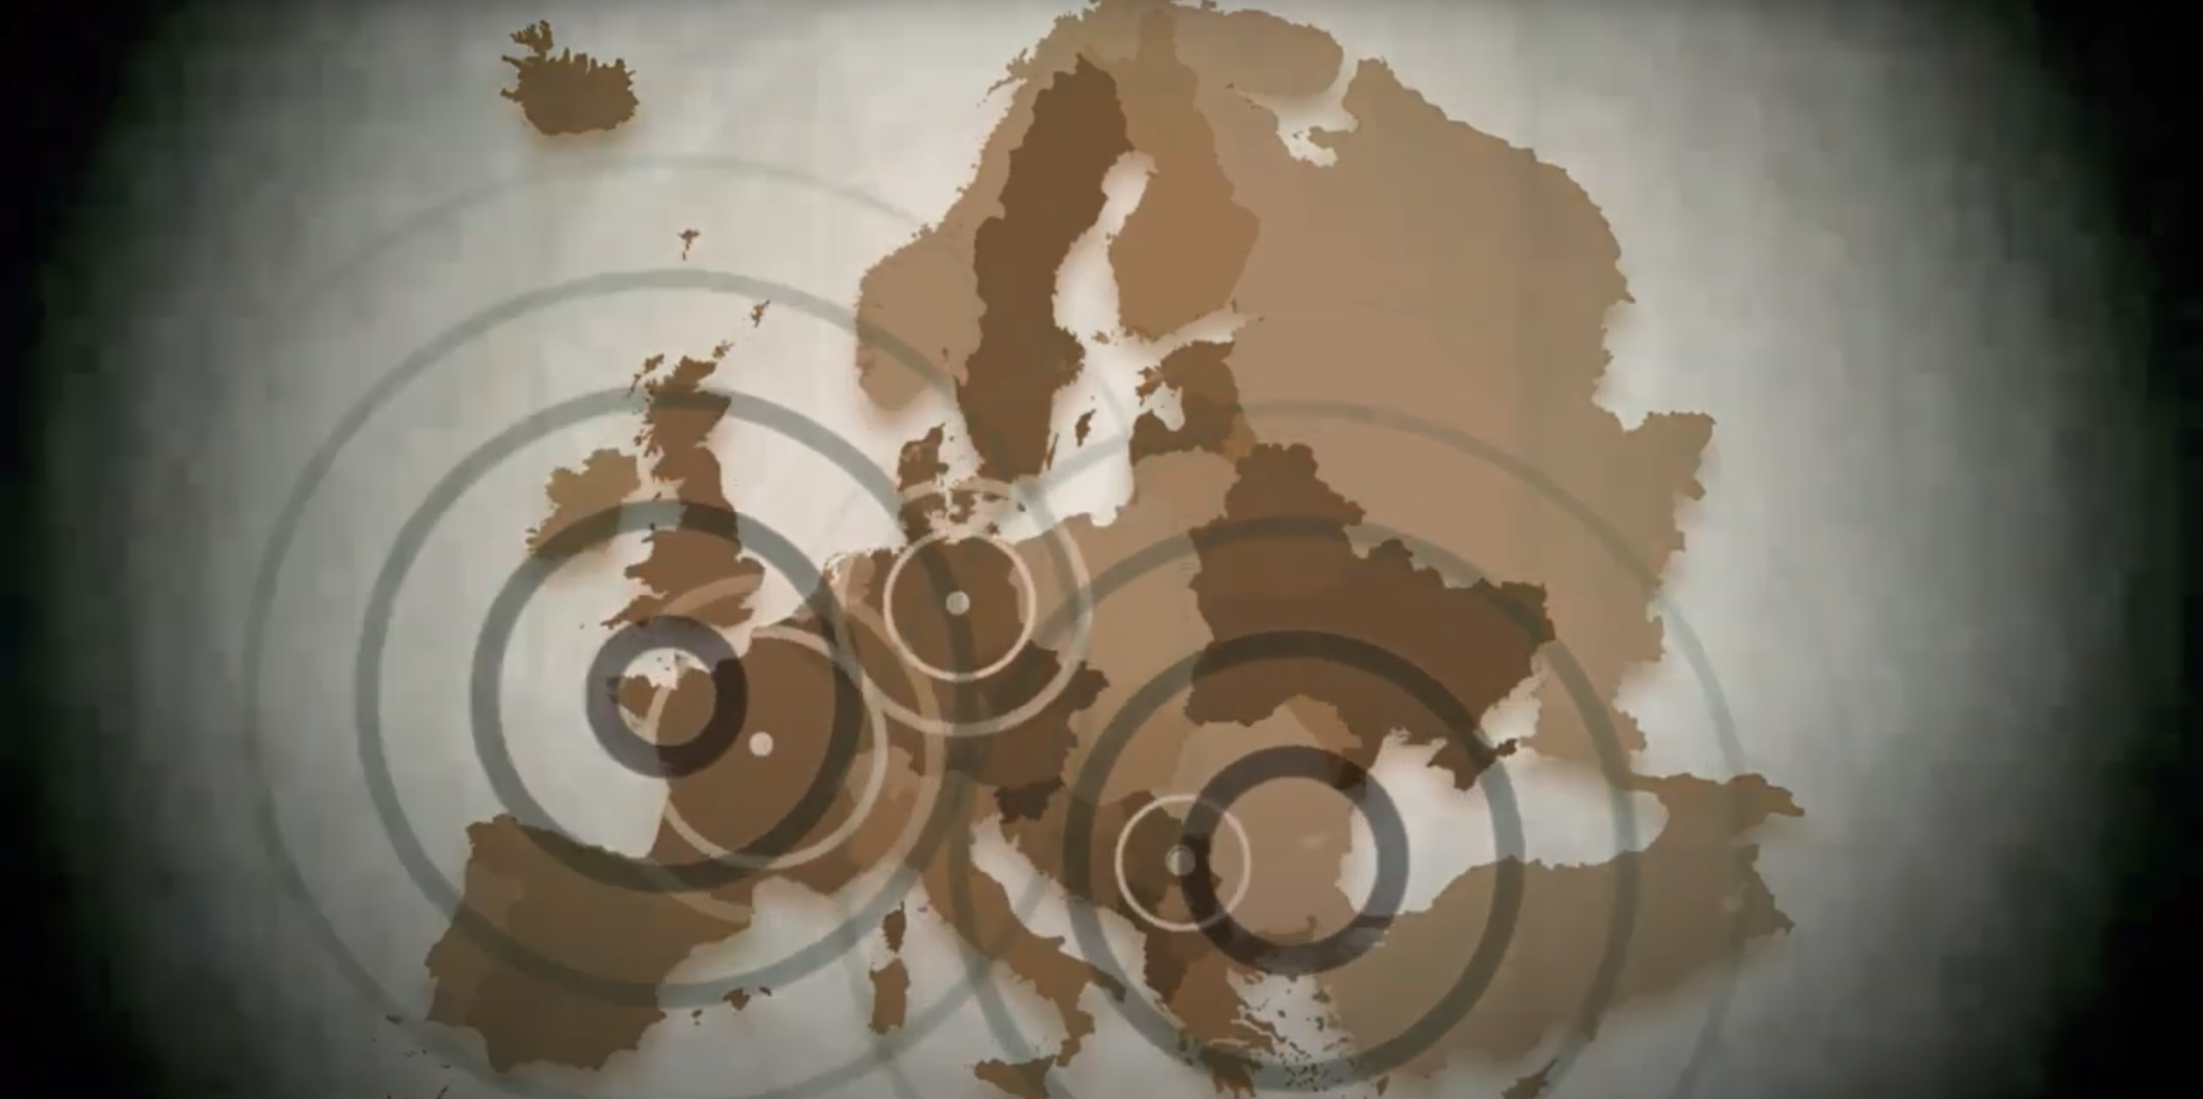
\includegraphics[width=.4\columnwidth]{Pictures/illu-propa.png}}
\end{wrapfigure}

\lgf{Dans les années 50, la télévision est devenue très populaire et presque tous les foyers ont acheté un téléviseur pour regarder leurs programmes préférés. Des réseaux de transmission dédiés ont été déployés partout sur la planète. En fait chaque type de communication avait son propre réseau un pour la radio un pour le téléphone un pour le télex,...}
\lge{In the 1950s, television became very popular and almost every household bought a television set to watch their favorite programs. Dedicated transmission networks were deployed all over the world. In fact each type of communication had its own network one for radio one for telephone one for telex,...}
 
\lgf{Dans les années 80, l'internet a vu le jour, mais les vitesses de transmission était faible et le réseau était limitée aux chargements de fichiers. Dans les années 90, des images et l'hypermédia avec le \ac{WWW} sont apparus, en lien avec l'augmentation des débits. Toujours dans les années 90, l'augmentation en puissance des microprocesseurs a permis la numérisation du signal télé. Les téléviseurs ont commencé à inclure des microprocesseurs et les réseaux sont passés d'une transmission analogique au numérique ; mais ils sont restés dédié à cet usage unique diffuser la télévision. Avec l'entrée dans le nouveau millénaire, l'internet a gagné en débit avec l'\ac{ADSL} et des fibres optiques. Il était possible d'intégrer des images dans les pages web mais la qualité était médiocre. Au même moment des centaines de canaux de télévision diffusaient en haute résolution leur programme via satellite ou par \ac{TNT}. De nos jours les communications internet ont gagné en vitesse et en qualité et certains pays ont coupé la \ac{TNT} et choisi de ne transmettre leurs programmes que par internet. En fait l'utilisation d'internet n'est pas uniquement un changement de réseau de distribution c'est aussi un changement majeur dans les usages et les applications. Vous pouvez regarder la télévision sur votre téléphone portable ou même regarder votre série favorite quand vous le voulez, à la demande. }
\lge{In the 80's, the internet was born, but the transmission speeds were low and the network was limited to file uploads. In the 90s, images and hypermedia with the \ac{WWW} appeared, in connection with the increase of the speeds. Also in the 90s, the increase in power of microprocessors allowed the digitization of the TV signal. Televisions started to include microprocessors and the networks went from analog to digital transmission; but they remained dedicated to this single use broadcasting television. With the entry in the new millennium, the Internet gained in speed with the \ac{ADSL} and optical fibers. It was possible to integrate images in web pages but the quality was poor. At the same time, hundreds of television channels were broadcasting their programs in high resolution via satellite or \ac{DTT}. Nowadays, Internet communications have gained in speed and quality and some countries have cut off DTT and chosen to transmit their programs only via Internet. In fact the use of the internet is not only a change in the distribution network but also a major change in the uses and applications. You can watch television on your cell phone or even watch your favorite series whenever you want, on demand.}



  \vspace{2em}

\lgf{\subsection{3 phases technologiques}}
\lge{\subsection{3 technological phases}}

   \vspace{1em}

\begin{wrapfigure}{r}{6cm}
\centerline{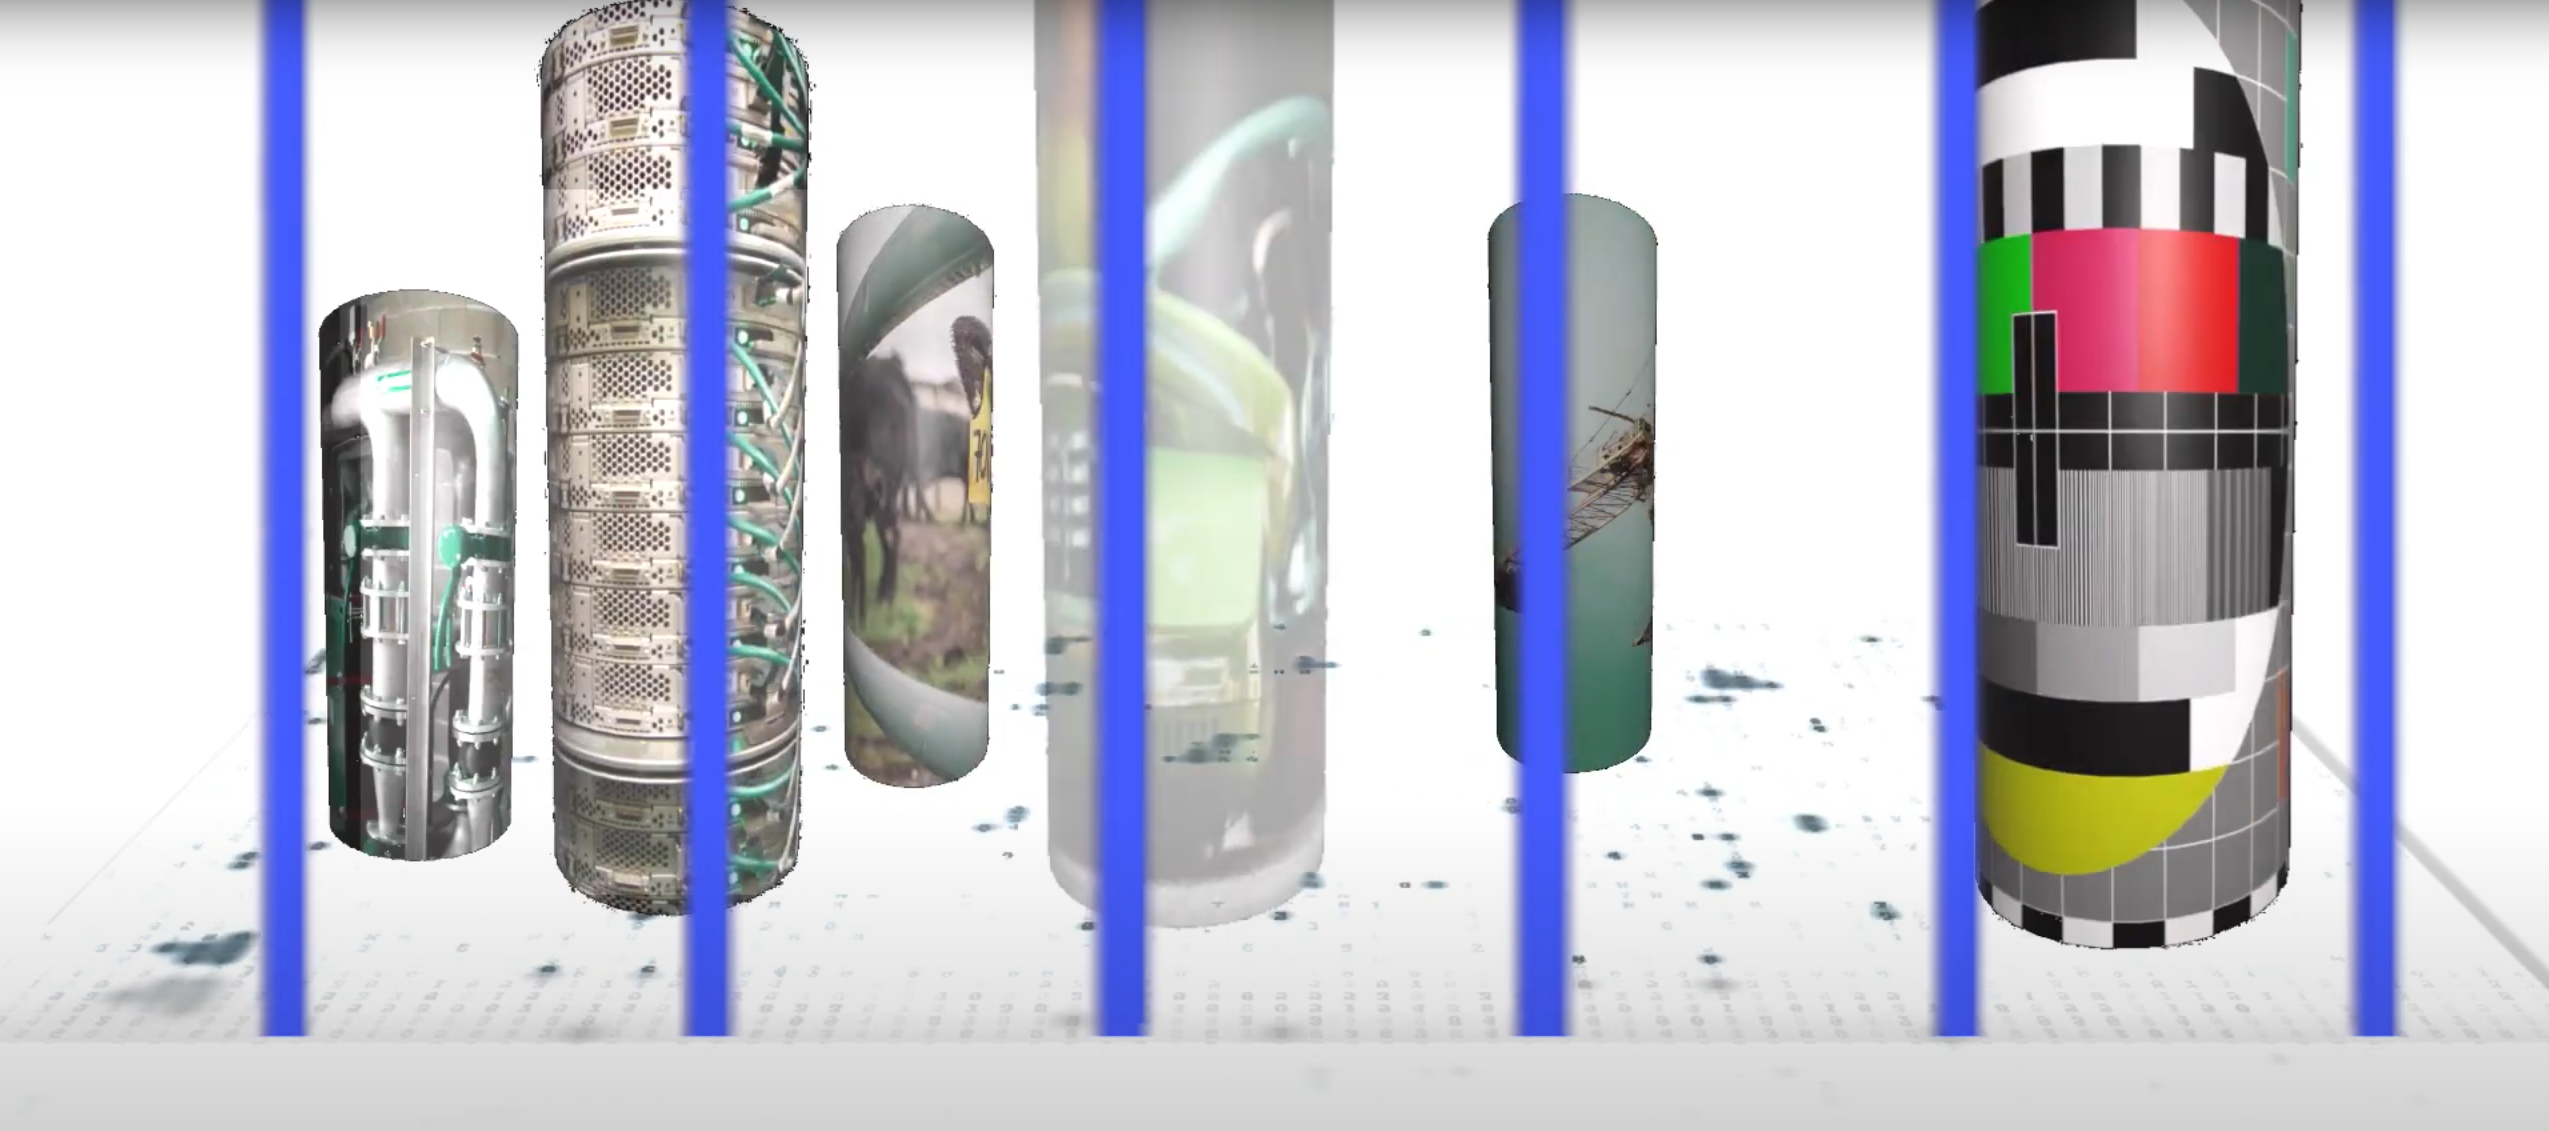
\includegraphics[width=.4\columnwidth]{Pictures/illu-verticals.png}}
\end{wrapfigure}
\lgf{De cet exemple, on peut définir trois phases dans le développement d'une technologie. Dans la première phase, un réseau spécifique est construit pour un usage bien défini. On appelle cela une approche \Index{verticale} ; une technologie est dédiée à un seul usage. Il est difficile d'échanger de l'information entre deux verticales. On fait aussi référence à des \Index{silos} car ils sont isolés. Dans une seconde phase, les verticales commencent à intégrer des technologies communes mais pas d'une manière coordonnée. Elles ne peuvent toujours pas communiquer facilement car elles n'ont pas fait les mêmes choix.}
\lge{From this example, we can define three phases in the development of a technology. In the first phase, a specific network is built for a well-defined use. This is called a \Index{vertical} approach; a technology is dedicated to a single use. It is difficult to exchange information between two verticals. We also refer to \Index{silos} because they are isolated. In a second phase, the verticals start to integrate common technologies but not in a coordinated way. They still cannot communicate easily because they have not made the same choices.}

~

\begin{wrapfigure}{r}{6cm}
\centerline{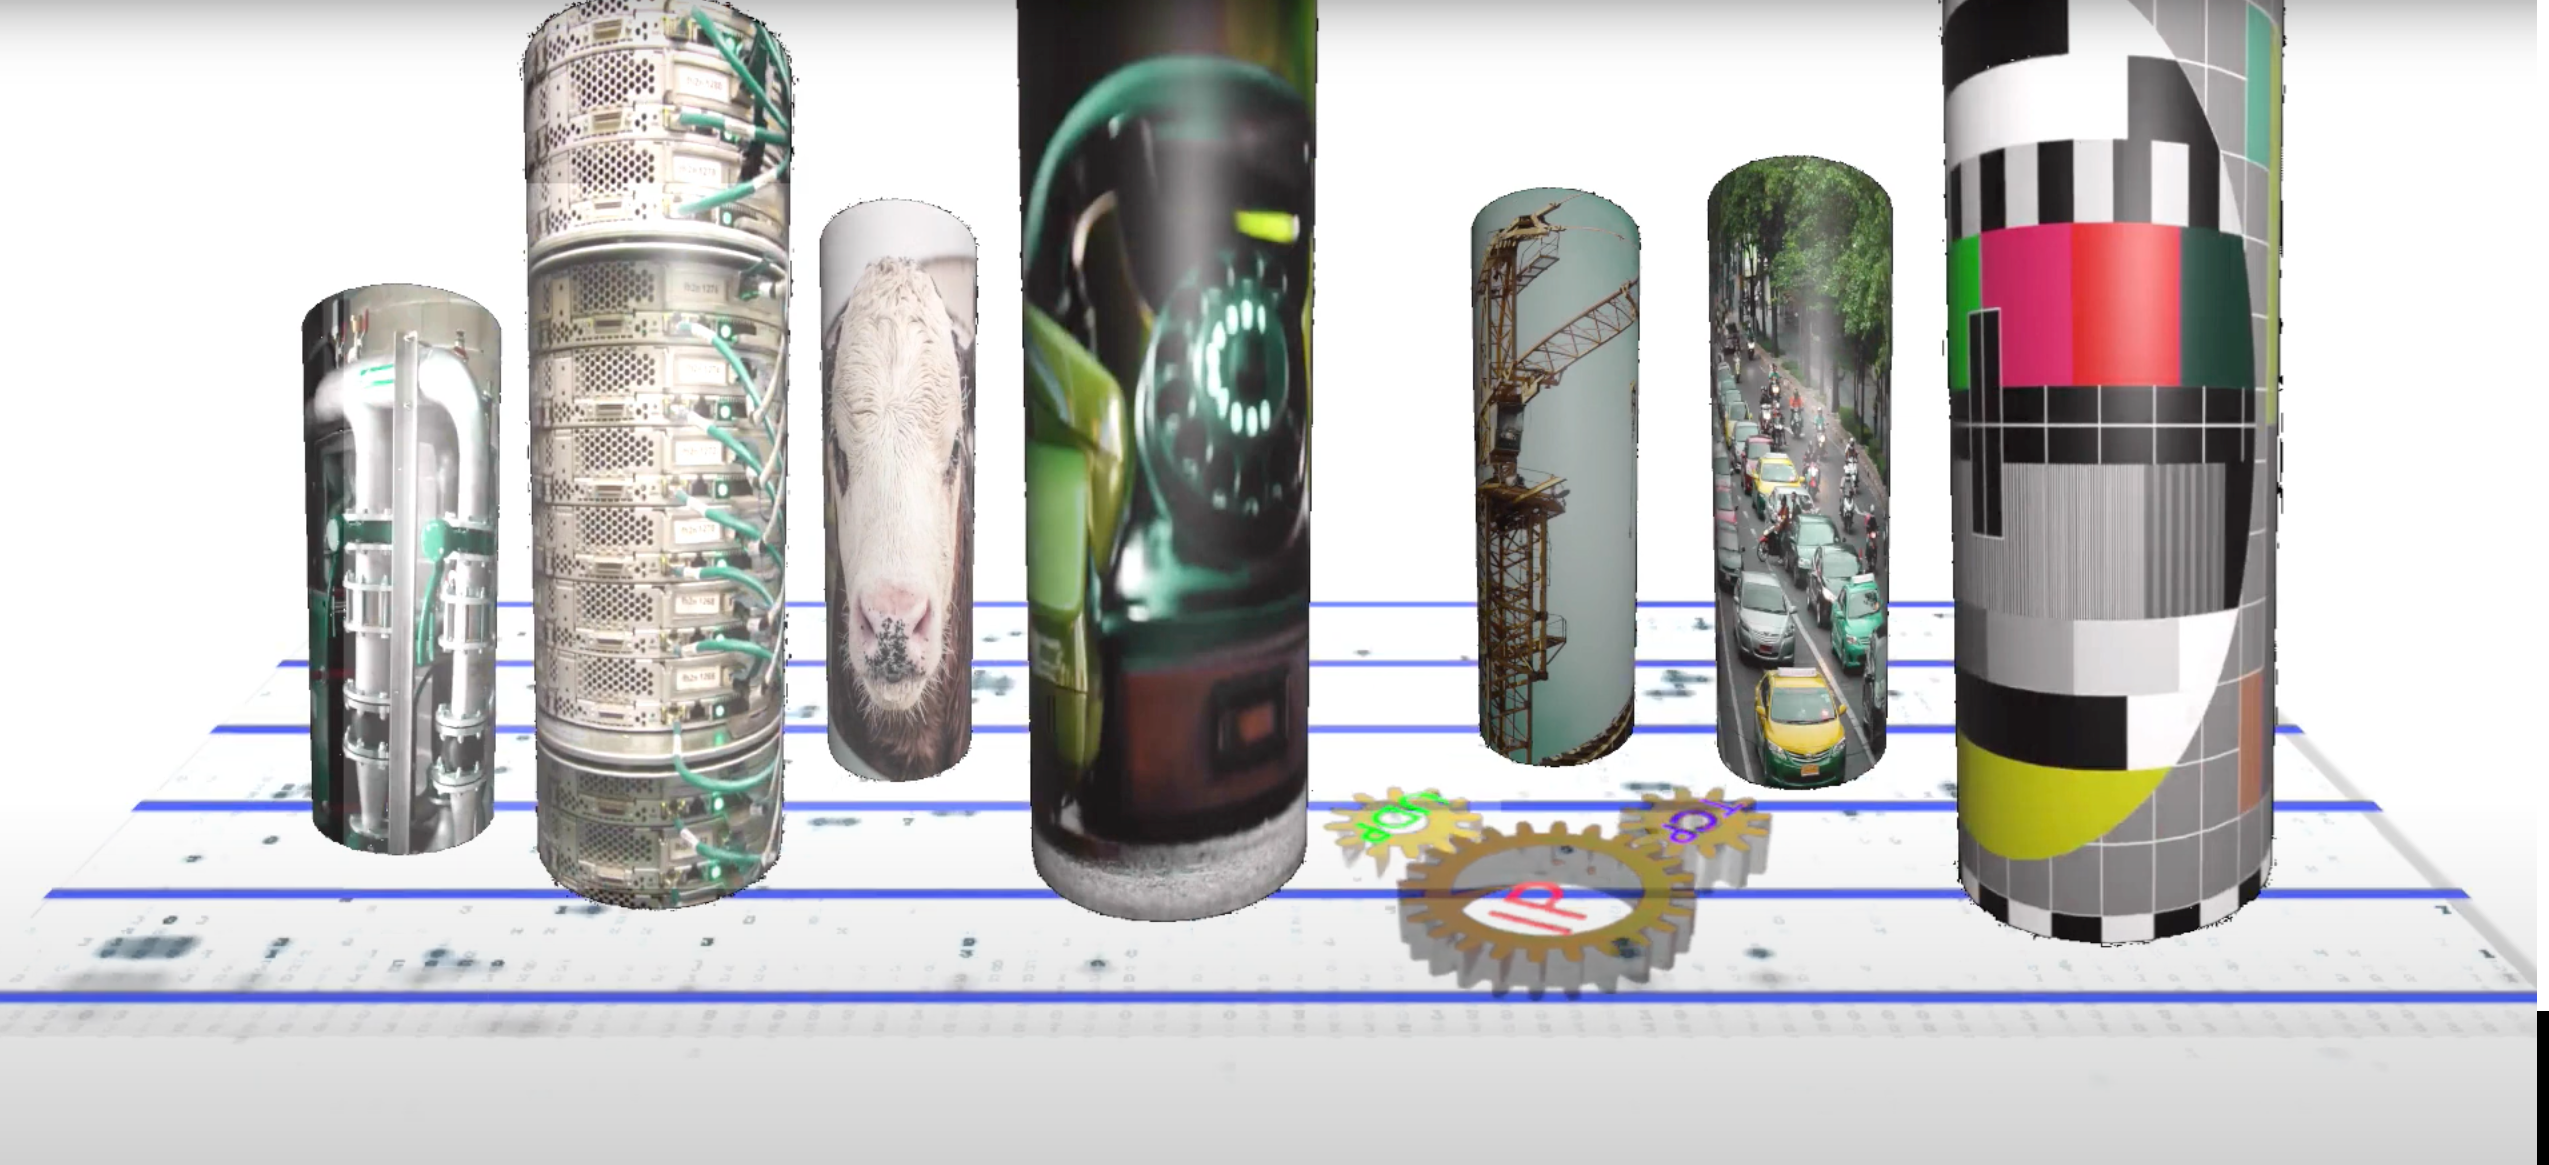
\includegraphics[width=.4\columnwidth]{Pictures/ill-horizontales.png}}
\end{wrapfigure}
\lgf{Dans une dernière phase, des verticales se coordonnent pour converger vers les mêmes technologies en définissant des règles et des usages communs. Ceci dans le but de réduire les coûts ou d'augmenter leur impact dans ce cas. On parle d'horizontal\index{Horizontale} car elle couvre plusieurs secteurs. L'internet est devenu une de ces horizontales pour beaucoup de services. L'internet des objets suit ce même mouvement. Des solutions particulières ont émergé pour résoudre des besoins spécifiques en agriculture, dans l'automobile, dans la santé, dans l'énergie. Quand les réseaux internet ont permis des communications à faible coût, l'architecture de l'internet a été prise en compte mais sans compatibilité. Le changement qu'on vit actuellement est la définition de fonctionnalités communes à différents domaines. Le but étant de réduire les coûts mais également de croiser les informations pour une meilleure gestion du processus industriel et un meilleur usage des ressources.}
\lge{In a final phase, verticals coordinate to converge on the same technologies by defining common rules and uses. This is done in order to reduce costs or to increase their impact in this case. We talk about \Index{horizontal} because it covers several sectors. The Internet has become one of these horizontals for many services. The Internet of Things follows this same movement. Particular solutions have emerged to solve specific needs in agriculture, in the automotive industry, in health, in energy. When Internet networks allowed low cost communications, the architecture of the Internet was taken into account but without compatibility. The change we are currently experiencing is the definition of common functionalities for different domains. The goal is to reduce costs but also to cross information for a better management of the industrial process and a better use of resources.}
 

  \vspace{2em}

\lgf{\section{L'Internet des Objets}}
\lge{\section{The Internet of Things}}


  \vspace{1em}
  
\lgf{Comment définir l’internet des objets~? Ou plutôt, quel internet des objets allons-nous étudier~? L’ambiguïté des deux termes "internet" et "objets" impose une définition plus précise ; ou du moins une classification pour mieux comprendre à quoi l’on fait référence.}
\lge{How do we define the Internet of Things? Or rather, which Internet of Things are we going to study? The ambiguity of the two terms "Internet" and "Things" requires a more precise definition; or at least a classification to better understand what we are referring to.}

  \vspace{1em}


\lgf{L’internet est maintenant totalement intégré dans nos vies, pour le travail, l’enseignement, pour les distractions. On l’utilise à la maison ou au travail sur nos ordinateurs, et on l'emporte avec nous de plus en plus avec nos smartphones. }
\lge{The internet is now totally integrated in our lives, for work, for education, for entertainment. We use it at home or at work on our computers, and we carry it with us more and more with our smartphones. }

\lgf{Chacun a sa définition de ce qu’est internet. Pour le grand public, il peut s’agir d’applications très populaires comme Facebook, Tik-Tok, Netflix, Zoom. Pour certains, un peu plus technophiles, l’internet peut être confondu avec le Web auquel on accède via Chrome ou Firefox. Les techniciens parleront de protocoles comme IP, TCP, HTTP, et d’adresses comme les adresses IP ou les URL.}
\lge{Everyone has their own definition of what the internet is. For the general public, it can be very popular applications like Facebook, Tik-Tok, Netflix, Zoom. For some, a little more technophile, the Internet can be confused with the Web which is accessed via Chrome or Firefox. Technicians will talk about protocols like IP, TCP, HTTP, and addresses like IP addresses or URLs.}

~~

\lgf{Comme ce livre est orienté technologie, notre approche relève plutôt de cette dernière catégorie. Nous verrons comment des protocoles développés il y a une vingtaine d’années pour des ordinateurs peuvent s’appliquer à d’autres dispositifs qu’il nous reste à définir.}
\lge{As this book is technology-oriented, our approach falls more into the latter category. We will see how protocols developed twenty years ago for computers can be applied to other devices that we have yet to define.}


\lgf{L'objectif de l'internet des Objets est de poursuivre l'intégration du réseau Internet pour permettre à autre chose que des ordinateurs d'échanger des données. Le but principal est d'optimiser les processus pour qu'ils soient plus efficaces pour économiser des ressources ou d'augmenter la productivité. Il s'agit donc d'un internet enfoui, loin du frigo ou de la montre connectés, qui vont remonter des informations avec une infrastructure ou d'autres équipements. On peut imaginer des capteurs dans une usine pour contrôler la production, des voitures connectées qui vont dialoguer pour éviter les collisions, la mesure du taux de remplissage des bennes de recyclage dans une ville pour optimiser les circuits de collecte, la surveillance du degré d'humidité d'un champ pour réduire la consommation d'eau...}
\lge{The goal of the Internet of Things is to further integrate the Internet to allow something other than computers to exchange data. The main goal is to optimize processes so that they are more efficient to save resources or increase productivity. It is therefore a buried internet, far from the fridge or the connected watch, which will bring back information with an infrastructure or other equipment. We can imagine sensors in a factory to control production, connected cars that will talk to each other to avoid collisions, measuring the filling rate of recycling bins in a city to optimize collection circuits, monitoring the degree of humidity in a field to reduce water consumption...}


\lgf{L’internet des Objets peut se résumer de la manière suivante : utiliser des protocoles développés pour des ordinateurs et maintenant des téléphones portables (plus puissants que les ordinateurs utilisés par l’internet à ses débuts) mais dans des environnements plus contraints. En effet, les lois de Moore, définissant les puissances de traitement des processeurs ainsi que la diminution continue des coûts de la mémoire, nous ont permis de doter les petits objets de ressources comparables à celles des ordinateurs d’il y a trente ans.}
\lge{The Internet of Things can be summarized as follows: using protocols developed for computers and now cell phones (more powerful than the computers used by the Internet in its early days) but in more constrained environments. Indeed, Moore's laws, defining the processing power of processors as well as the continuous decrease of memory costs, have allowed us to provide small objects with resources comparable to those of computers of thirty years ago.}

\lgf{L’internet des Objets, c’est résoudre l’équation suivante : continuer à faire la même chose car tous les systèmes d’information actuels utilisent les mêmes principes mais le faire différemment car ces principes sont trop coûteux en énergie, en temps de calcul et échange de données.}
\lge{The Internet of Things means solving the following equation: continue to do the same thing because all current information systems use the same principles but do it differently because these principles are too costly in terms of energy, computing time and data exchange.}

\lgf{L’\ac{IoT}, l’internet des objets ou des choses, est une architecture globale permettant à des objets (équipements de même type ou non), d’interagir de manière autonome via internet. Cette interaction~:}
\lge{The \ac{IoT} is a global architecture allowing objects (equipment of the same type or not) to interact autonomously via the Internet. This interaction:}

\begin{itemize}
    \item 
        \lgf{est réalisée, par construction, au travers d’un réseau internet, ce qui implique généralement que les objets/choses soient pourvus d’une adresse IP~;}
        \lge{is realized, by construction, through an Internet network, which generally implies that the objects/things are provided with an IP address;}
        
    \item 
        \lgf{est relatif à des commandes (opérations de contrôles ou appels de fonctions) ou des échanges de données ou d’informations.}
        \lge{is related to commands (control operations or function calls) or data or information exchanges.}
\end{itemize}

  \vspace{1em}


\lgf{Ce nouveau paradigme \ac{STIC} qu’est l’IoT est une convergence de nombreux domaines d’applications tels que : les maisons ou bâtiments intelligents, les villes du futur, l’industrie du futur (industrie 4.0), l’énergie, les systèmes de transport, l’agriculture, la eSanté, etc., vers une suite protocolaire réduite, interopérable et sécurisée. Le mouvement est en marche et, vu le nombre d'acteurs concernés, va prendre plusieurs années. Mais les bases sont déjà bien établies et c'est ce que vous allez apprendre dans cet ouvrage.}
\lge{The new IoT paradigm is a convergence of many application domains such as: smart homes or buildings, cities of the future, industry of the future (industry 4.0), energy, transportation systems, agriculture, eHealth, etc., towards a reduced, interoperable and secure protocol suite. The movement is underway and, given the number of players involved, will take several years. But the foundations are already well established and that's what you'll learn in this book.}

 \vspace{2em}
 
\section{Le problème}

  \vspace{1em}

\lgf{Un des problèmes que rencontre l’internet des objets, c’est que l’IoT ne démarre pas ex-nihilo. Maintenant que les technologies qui ont fait le succès de l'Internet sont matures, il ne s'agit pas juste de les appliquer à un nouveau domaine. Des objets étaient capables de communiquer bien avant qu’internet n’existe. Chaque secteur a déjà développé ses solutions, plus ou moins standards, plus ou moins propriétaires.}
\lge{One of the problems with the Internet of Things is that the IoT doesn't start ex-nihilo. Now that the technologies that made the Internet successful are mature, it's not just a matter of applying them to a new domain. Objects were able to communicate long before the Internet existed. Each sector has already developed its solutions, more or less standard, more or less proprietary.}


\lfg{La figure~\vref{fig-bazar} reprend un certain nombre de travaux et de groupes qui spécifient les protocoles pour l’internet des objets. }
\lge{The figure~\vref{fig-bazar} lists a number of works and groups that specify protocols for the Internet of Things. }


\begin{figure}[tbp]
\centerline{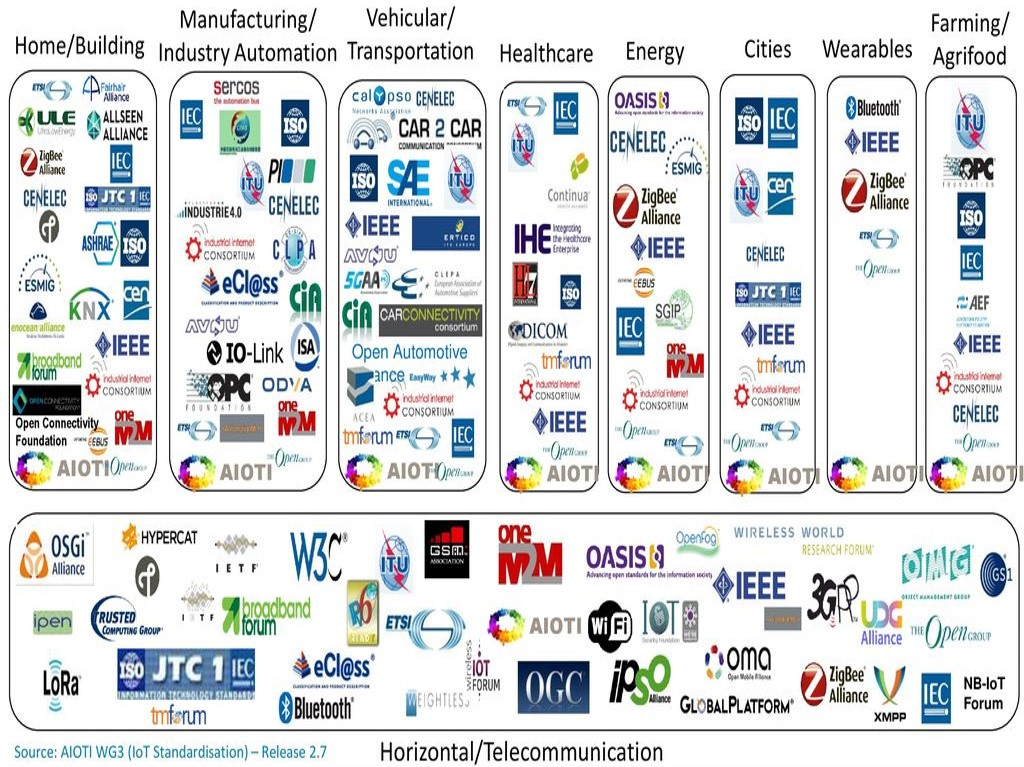
\includegraphics[width=1\columnwidth]{Pictures/IOTBazar_Domaines.jpeg}}
\lgf{\caption{Quelques standards de l'IoT}}
\lge{\caption{Some IoT standards}}
\label{fig-bazar}
\end{figure}

\lgf{Sans entrer dans les détails, on voit que certains logos se retrouvent à plusieurs emplacements, qu’il y a pour chaque secteur une profusion de solutions qui nuisent à l’interopérabilité et aux évolutions. L’internet des objets, dans son acception la plus large, consiste à simplifier cette architecture, comme l’internet l'a fait il y a quelques années dans le domaine des télécoms en simplifiant ce modèle et en permettant à ces différents acteurs de converger vers une architecture commune et un ensemble de solutions plus réduit.}
\lge{Without going into detail, we can see that some logos are found in several places, that there is a profusion of solutions for each sector that hinders interoperability and evolution. The Internet of Things, in its broadest sense, is about simplifying this architecture, just as the Internet did a few years ago in the telecoms sector, by simplifying this model and enabling these different players to converge on a common architecture and a smaller set of solutions.}

\lgf{Cela ne veut pas nécessairement dire moins d’acteurs, mais une plus grande cohérence dans les choix technologiques.}
\lge{This does not necessarily mean fewer players, but greater consistency in technological choices.}

\lgf{La figure~\vref{fig-bazar-OS} analyse l’IoT par domaine d’application en se focalisant sur la composante réseau. L’IoT et les objets connectés sont des systèmes complexes pour lesquels les solutions open source, les alliances entre industriels, les organismes de standardisation sont toujours fragmentés ; cependant de manière moins importante, montrant que la structuration est en marche.}
\lge{The figure~\vref{fig-bazar-OS} analyzes the IoT by application domain, focusing on the network component. IoT and connected objects are complex systems for which open source solutions, alliances between manufacturers, and standardization bodies are still fragmented; however, to a lesser extent, showing that structuring is underway.}

\begin{figure}[tbp]
\centerline{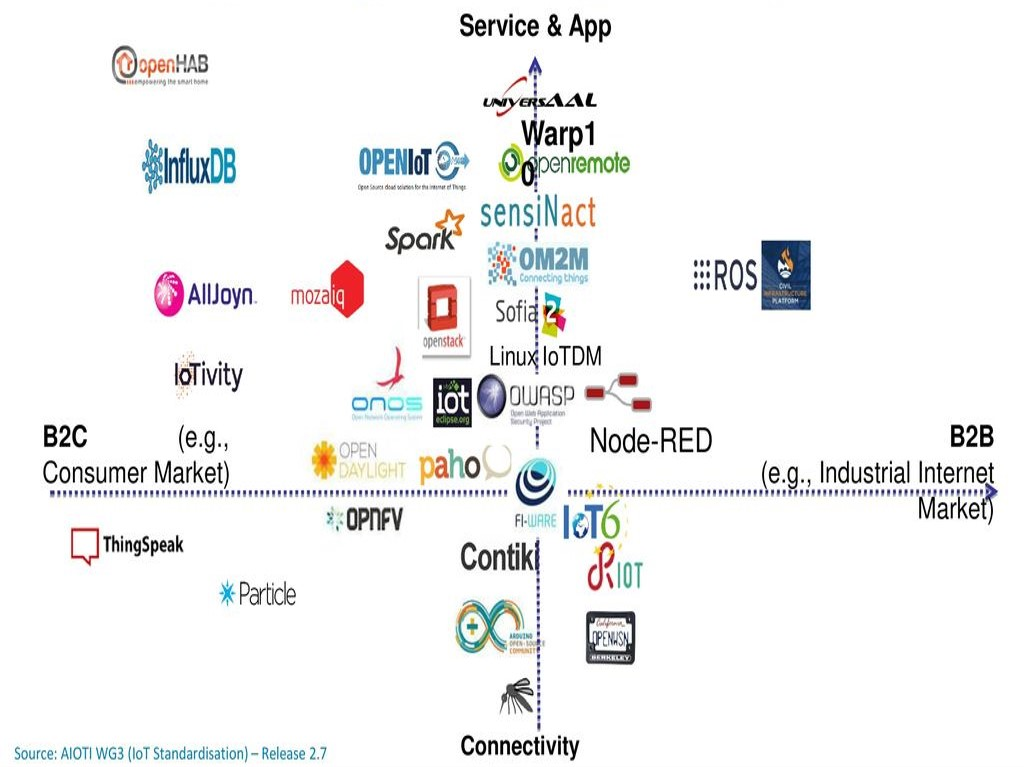
\includegraphics[width=1\columnwidth]{Pictures/IOTBazar_OpenSources.jpeg}}
\lgf{\caption{Quelques applications Open Source pour l'IoT}}
\lge{\caption{Some open source applications for the IoT}}

\label{fig-bazar-OS}
\end{figure}

\lgf{Cette fragmentation de l’écosystème est paradoxale. Si l’on résume sommairement, les solutions proposées reviennent à interroger un équipement sur le terrain pour accéder à une valeur, la traiter et renvoyer une commande pour interagir avec l’environnement.}
\lge{This fragmentation of the ecosystem is paradoxical. If we summarize, the proposed solutions amount to interrogating a piece of equipment in the field to access a value, process it and send back a command to interact with the environment.}

\lgf{Pourquoi cette foison de solutions différentes~? Cela peut venir des besoins de fiabilité, de sécurité, de portée de la donnée, mais cela vient aussi de l’histoire. La communication avec des Objets est tout aussi ancienne que la communication entre ordinateurs (qui sont eux-mêmes des Objets). Mais à l’époque, chaque domaine a suivi sa propre voie en spécialisant les solutions pour répondre à ses besoins propres. Il en résulte des solutions optimisées pour un domaine particulier. Mais chaque fois qu’il faut modifier une technologie, le travail doit être adapté pour chaque domaine, introduisant des coûts et des délais supplémentaires.}
\lge{Why are there so many different solutions? It may come from the needs of reliability, security, data scope, but it also comes from history. Communication with Things is just as old as communication between computers (which are themselves Things). But at the time, each field went its own way, specializing solutions to meet its own needs. The result is solutions optimized for a particular domain. But every time a technology has to be modified, the work has to be adapted for each domain, introducing additional costs and delays.}

\lgf{De même, chaque domaine ayant sa propre représentation des données, il est relativement difficile de les combiner pour avoir une vision plus globale. On arrive donc à des systèmes fermés, chers, peu évolutifs, mais optimisés pour les tâches qu’ils ont à réaliser.}
\lge{Also, since each domain has its own data representation, it is relatively difficult to combine them to have a more global vision. We therefore end up with closed systems, expensive, not very scalable, but optimized for the tasks they have to perform.}


\lgf{Au fil du temps, les protocoles de l’internet ont pu être utilisés, mais il s’agit surtout de complémenter les technologies existantes sans qu’il soit possible d’interconnecter deux domaines.}
\lge{Over time, the protocols of the Internet could be used, but it is mainly a matter of complementing existing technologies without it being possible to interconnect two domains.}



  \vspace{2em}

\lgf{\section{Evolution de l'IoT}}
\lge{\section{IoT evolution}}


  \vspace{1em}

\lgf{L’exemple de l’évolution du réseau de télévision est éloquent. À ses débuts, ce réseau est analogique et hautement spécialisé pour diffuser les programmes transportés sur des signaux analogiques sur des équipements spécialisés, les téléviseurs.}
\lge{L’exemple de l’évolution du réseau de télévision est éloquent. À ses débuts, ce réseau est analogique et hautement spécialisé pour diffuser les programmes transportés sur des signaux analogiques sur des équipements spécialisés, les téléviseurs.}

\lgf{Avec les progrès des processeurs informatiques, il devient possible de transporter les données en utilisant un codage numérique. Mais des réseaux spécialisés restent nécessaires, l’Internet n’offrant pas la même qualité.}
\lge{With the progress of computer processors, it becomes possible to transport data using digital coding. But specialized networks are still needed, as the Internet does not offer the same quality.}



\lgf{La dernière étape consiste à intégrer ces flux dans l’internet classique. Cela devient possible par la montée en débit des réseaux filaires et radio (Wi-Fi, 4G...). }
\lge{The last step consists in integrating these flows into the traditional Internet. This becomes possible by increasing the speed of wired and radio networks (Wi-Fi, 4G...). }


\lgf{Cette mutualisation des accès via l’internet permet non seulement une réduction des coûts, mais aussi l'apparition de nouveaux usages comme la télévision sur les téléphones portables ou les séries à la demande.}
\lge{This pooling of accesses via the Internet allows not only a reduction of costs, but also the appearance of new uses such as television on cell phones or series on demand.}

\lgf{L’internet des Objets suit la même voie. En plus des technologies spécifiques, les protocoles de l’internet sont intégrés, mais en les adaptant aux contextes du secteur.  Nous sommes actuellement en train de vivre la convergence vers un ensemble réduit de protocoles, une standardisation de la représentation de la donnée, et son traitement sur des plates-formes plus génériques. }
\lge{The Internet of Things follows the same path. In addition to specific technologies, the protocols of the Internet are integrated, but adapted to the contexts of the sector.  We are currently experiencing the convergence towards a reduced set of protocols, a standardization of data representation, and its processing on more generic platforms.}

\lgf{Le déclencheur n’est pas la montée en débit comme pour la télévision, mais la possibilité d'avoir des équipements peu chers, aux capacités réduites par rapport à l'informatique traditionnelle et autonomes énergétiquement, tout en ayant une meilleure intégration dans les systèmes d'information actuels.  }
\lge{The trigger is not the increase in speed as for television, but the possibility of having inexpensive equipment, with reduced capacities compared to traditional computing and energy autonomous, while having a better integration in the current information systems.  }


  \vspace{2em}

\section{Des objets contraints}

  \vspace{1em}

Avec les progrès de l’électronique, les processeurs deviennent de plus en plus puissants et les super-ordinateurs d’hier sont maintenant dans une montre ou un smart-phone. 

Pour l’internet des objets, la logique est un peu différente. La loi de Moore va induire une réduction des coûts de fabrication plutôt qu'une augmentation des puissances de traitement. Le principal critère pour un internet des objets massif reste l’énergie ; connecter un appareil à une source d’énergie ou recharger une batterie a un coût. Augmenter la vitesse du processeur ou la taille de la mémoire induit une plus grande consommation d’énergie de l'objet. On peut donc s’attendre à une certaine stabilité des performances des objets car ceux-ci resteront limités en performances.

Les objets sont généralement limités en termes de puissance de traitement, de mémoire et d’énergie. Selon le standard de l’IETF \rfc{7228}, les dispositifs peuvent être répartis en trois classes qui se retrouvent aussi dans la segmentation des processeurs :

\begin{itemize}
\item La classe 0, avec moins de 10 ko de mémoire volatile pour stocker les données temporaires et 100 ko de mémoire Flash pour stocker le code informatique de l'objet. C'est l’équivalent d’un Arduino UNO (2 ko de RAM et 32 ko de Flash). Il est presque impossible d’installer à la fois les protocoles utilisés pour communiquer sur Internet (même de manière restreinte) et les applications qui tournent dessus. 
\item La classe 1 a environ 10 Ko de RAM et 100 Ko de Flash. Avec une adaptation, il est possible d’y installer une pile IP. Il s'agit par exemple d'équipement comme le Pycom Lopy4 que nous utiliserons par la suite (et qui se situe dans la limite haute) sur lequel le système d'exploitation est minimal. Ainsi, le Pycom utilise une version simplifiée du langage Python (micro-python) qui permet de l'adapter à la limitation du système.
\item La classe 2 est moins restreinte avec au moins 50 ko de RAM et 250 ko de Flash (comme un Raspberry Pi). Le système d’exploitation Linux peut fonctionner sur ces appareils. Par conséquent, il y a peu de limitations sur la pile IP et les applications s’y exécutant.
Les appareils de classe 1 ont trop de restrictions pour utiliser les protocoles définis pour des objets plus gros. L’\ac{IETF}, l'organisme qui standardise les protocoles de l'internet, a proposé une révision de sa pile de protocoles afin d’adapter sa pile protocolaire à un environnement contraint.
\end{itemize}


La figure~\vref{fig-encap} résume les moyens d'interconnexion suivant la classe de l'objet~:
Un appareil de classe 0 ne peut pas utiliser directement l’internet pour échanger des informations, d’où la nécessité d’installer une passerelle pour capter le trafic et l’envoyer sur l’internet. Il ne possède pas directement d'adresse IP. Les passerelles LoRaWAN \ac{LNS} et \acs{3GPP} \ac{SCEF} agissent dans ce sens (nous reviendrons là-dessus). Les données produites sont encapsulées par ces passerelles dans des protocoles comme \ac{HTTP} ou \ac{MQTT}, que nous verrons également dans la suite du cours.

Les appareils de classe 1 peuvent aussi utiliser une passerelle pour s’interconnecter à l’internet traditionnel, mais plutôt que d'encapsuler les données produites dans d'autres protocoles comme le fait la classe 0, les passerelles pour les appareils de classe 1 vont traduire un protocole contraint dans son équivalent dans le monde non contraint.

Les dispositifs de classe 2 peuvent interagir directement avec d’autres nœuds sur l’internet, sans passer par une passerelle.

\begin{figure}[tbp]
\centerline{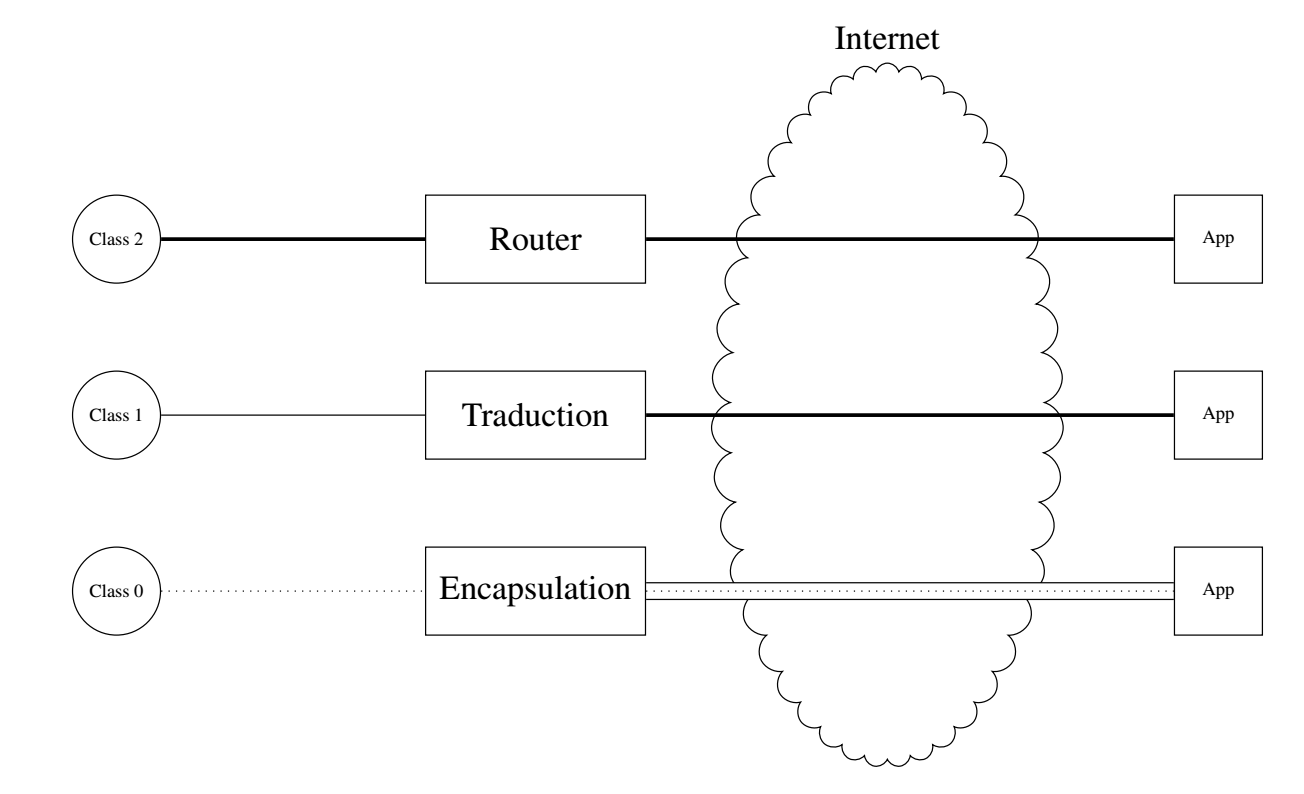
\includegraphics[width=1\columnwidth]{Pictures/Encpasul.png}}
\caption{Possibilités d'interconnection}
\label{fig-encap}
\end{figure}

  \vspace{2em}

\section{L'interopérabilité}

  \vspace{1em}


Un autre défi concerne le nombre de dispositifs. Certaines études prévoient 500 milliards de dispositifs à la fin de la décennie.

  \vspace{1em}
 \begin{wrapfigure}{r}{3cm}
\Youtube{https://youtu.be/2TQiTskfZtc}
\end{wrapfigure}
Avec cet énorme internet des objets, où presque chaque équipement comprendra des éléments de détection ou d’action, l’intégration dans un système d’information deviendra un véritable défi. Comme l’internet des objets actuel est conçu pour une verticale (c'est-à-dire pour des applications spécifiques), les dispositifs sont choisis et intégrés au moment de la conception du système. Les ingénieurs choisissent leurs capteurs, connaissent précisément leurs caractéristiques et écrivent leur code en fonction de ce qu'ils ont intégré. 

L’internet des objets massif change la donne. Les dispositifs ou les choses ne peuvent pas être intégrés dès le départ dans un système d’information statique. L’intégration doit se faire au fil du temps et doit gérer les évolutions des dispositifs pendant longtemps (les fabricants de dispositifs peuvent changer, les produits évolueront avec de nouvelles fonctionnalités, etc.)

Cette question d’interopérabilité a été formalisée dans le modèle \ac{LCIM}~\cite{tolk2003levels} (voir figure~\vref{fig-lcim}) peut être représenté par un compteur pour mesurer le degré d'interopérabilité.

\begin{figure}[tbp]
\centerline{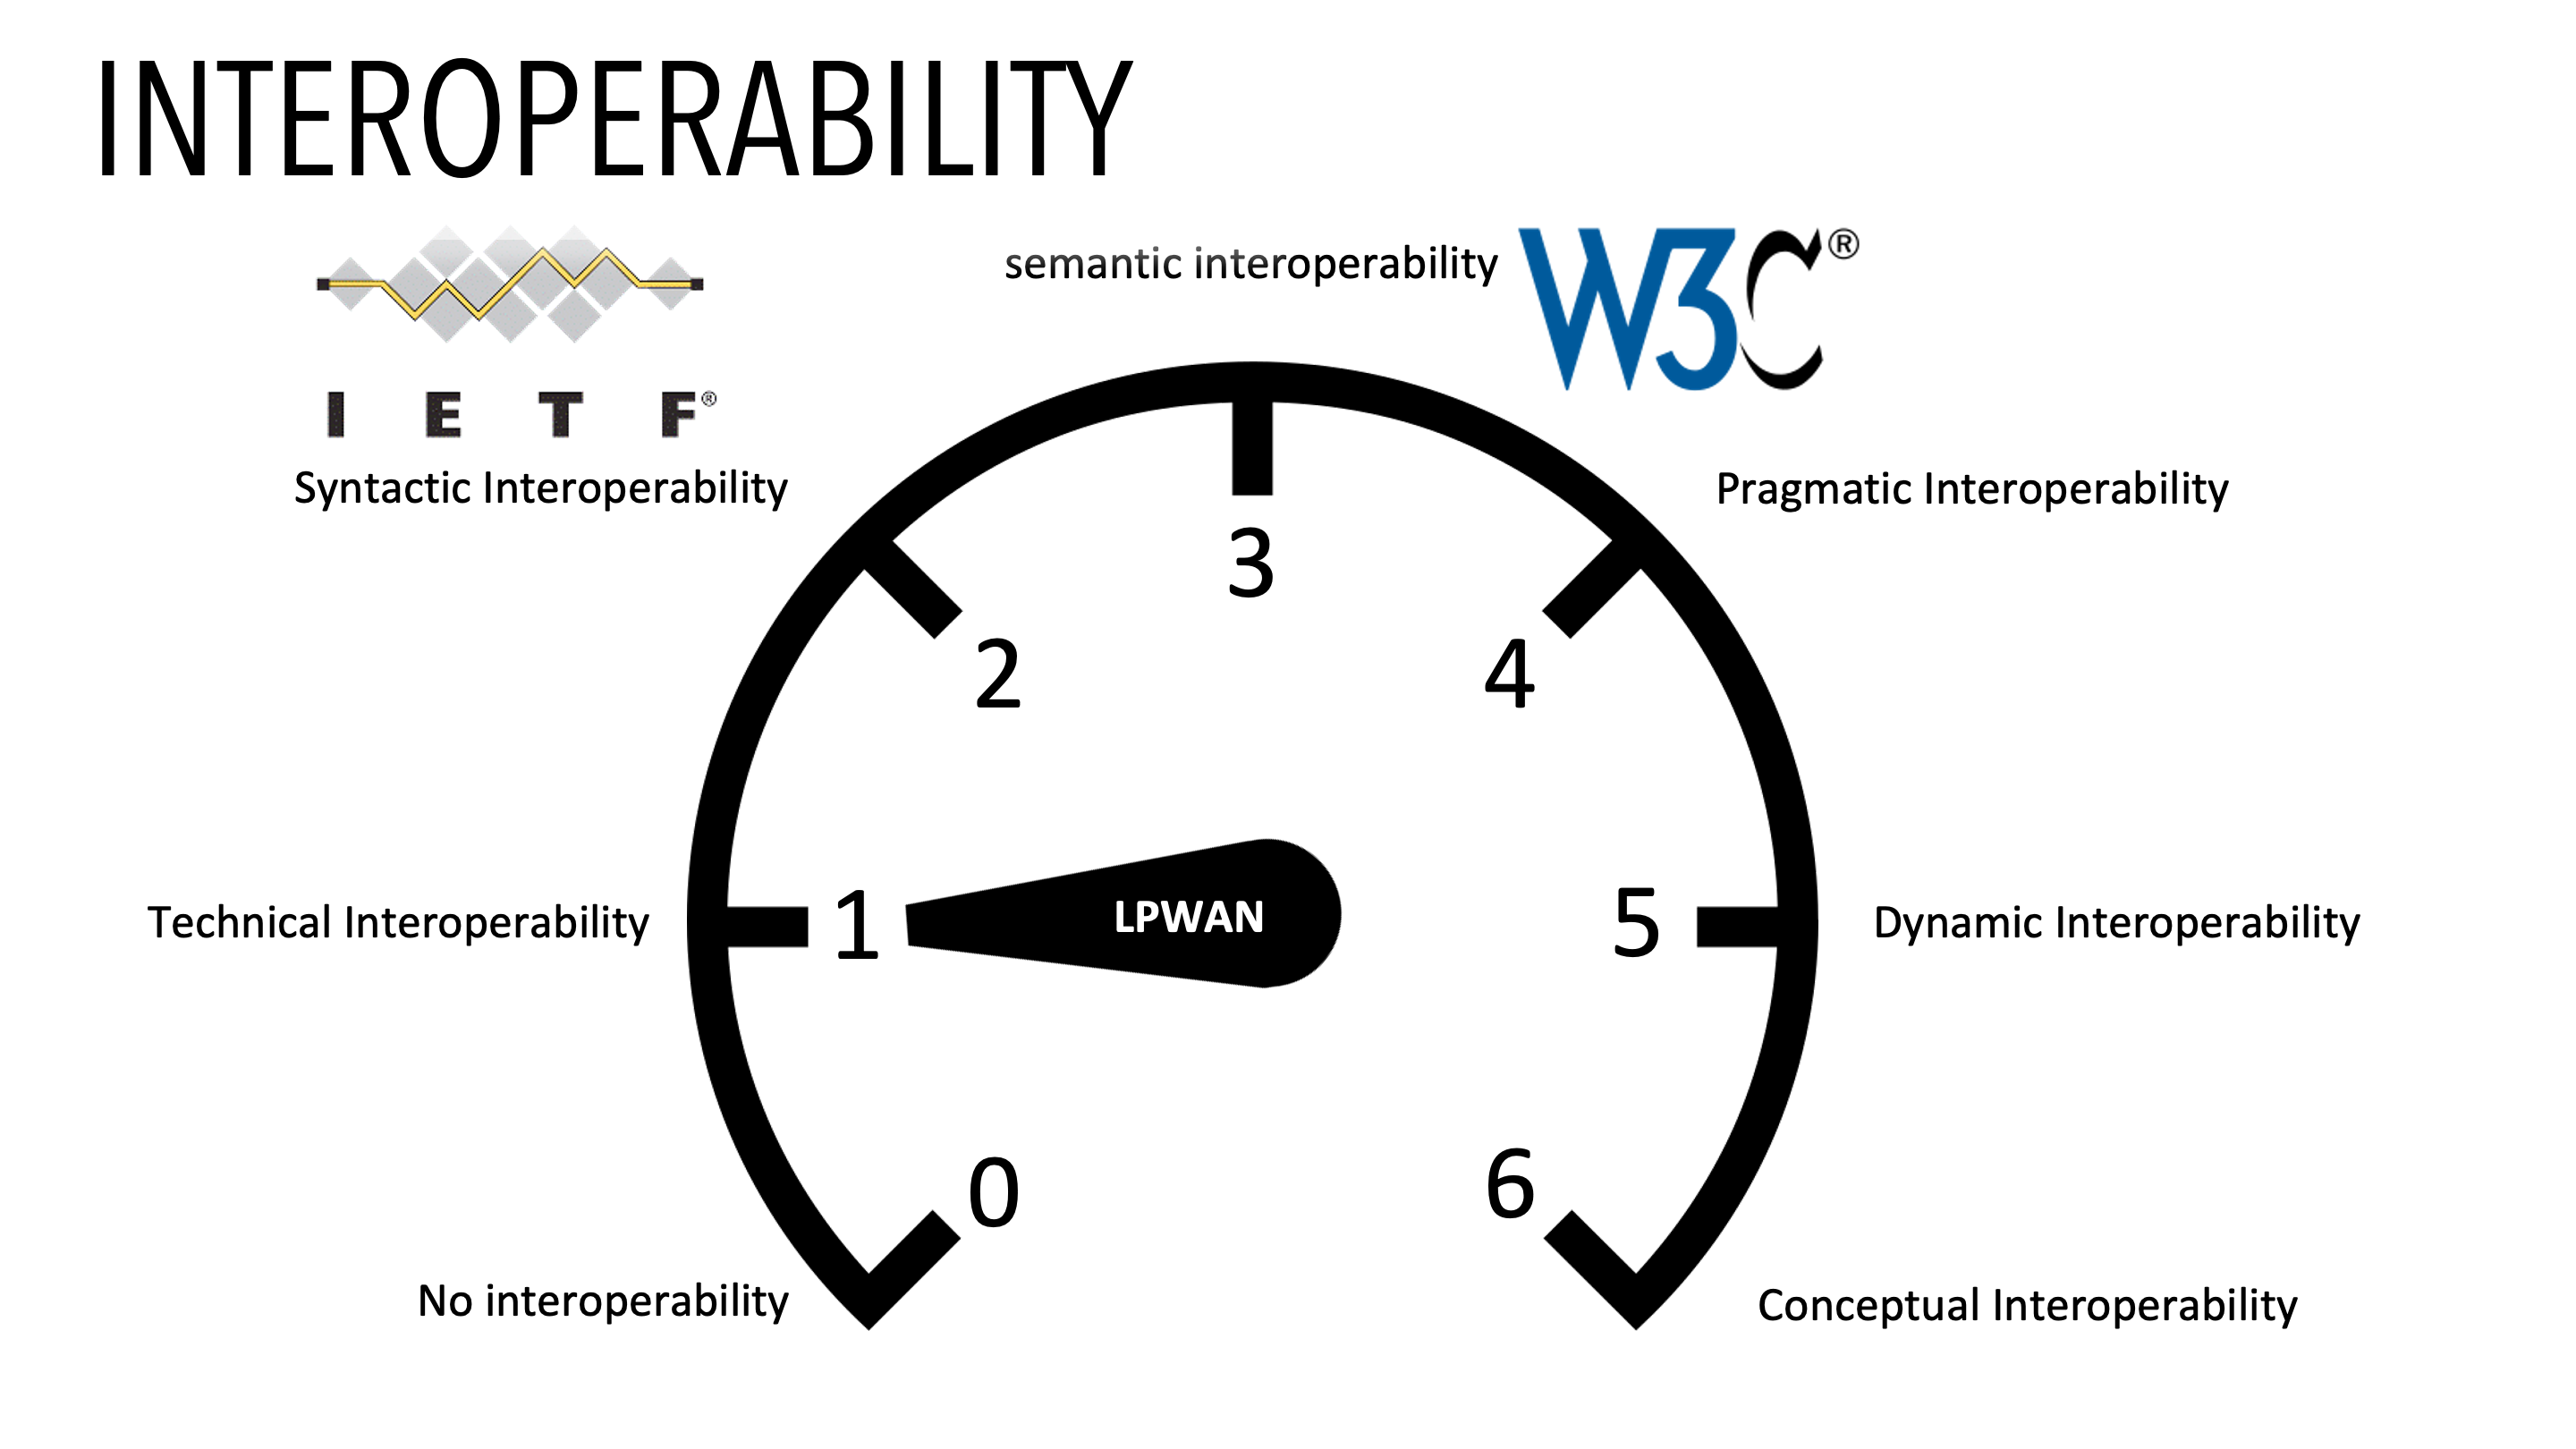
\includegraphics[width=1\columnwidth]{Pictures/TPT2020.png}}
\caption{Niveau d'interopérabilité}
\label{fig-lcim}
\end{figure}


Il distingue six niveaux d’interopérabilité, parmi lesquels :

\begin{itemize}
     \item Au niveau zéro, on n'est pas connecté ; on ne parle à personne donc on n'a pas de problèmes d'interopérabilité. 
    \item  Au niveau 1, on est capable de transmettre de l'information,  mais il faut que les deux côtés connaissent les règles. On a un système intégré ; les applications doivent  connaître précisément les spécifications des objets avec lesquels ils communiquent,  car elles définissent ses propres formats des échanges de données. On pourrait prendre l'exemple qu'une carte électrique où un processeur communique avec des capteurs via un circuit imprimé. Le code tournant sur le processeur peut être écrit à l'avance car il y a peu de chance qu'un utilisateur dessoude les composants pour les remplacer par d'autres. Cela correspond à l'encapsulation, si l'on considère les objets en réseau de la figure~\vref{fig-encap}, l'élément d'interconnexion doit être configuré pour en fonction de l'objet émetteur encapsuler les données vers la bonne application chez le bon récepteur. 
    \item L’interopérabilité syntaxique (niveau 2) où deux nœuds peuvent échanger des données, sans être a préalable configurés pour cet échange. C'est le cas de l'Internet. En utilisant cette suite de protocoles, en ayant une adresse valide sur le réseau, toute application est capable d'échanger des données avec une autre. En revanche, les données que vous allez échanger sont propres à une application. Les vidéoconférences sont un très bon exemple d'interopérabilité de niveau 2. Vous ne pouvez pas utiliser Zoom si votre correspondant utilise Teams car les formats sont différents. L'\ac{IETF}  est le regroupement de différents acteurs (industriels, académiques,...) qui produisent les standards liés à ce réseau. Il se reconnaissent par l'acronyme \ac{RFC} suivi d'un nombre. 
    \item L’interopérabilité sémantique (niveau 3) implique que le récepteur est capable d'interpréter les données reçues.Le web est un très bon exemple d'interopérabilité de niveau 3. Quel que soit votre navigateur, vous pouvez afficher les pages d'un site web et suivre les liens. Le sens de l'information est compris de la même manière des deux côtés. Pour le Web, le format \ac{HTML} permet à l'aide de balises (mots-clés) de structurer un texte en y ajoutant des informations de formatage ou des liens vers d'autres documents. Le W3C définit les standards.
     \item Les niveaux supérieurs d'interopérabilité vont être lié à la précision du modèle qui va représenter le système.     
\end{itemize}


L'internet qu'on connaît est une très bonne illustration du besoin d'interopérabilite. Il a permis, grace à une uniformisation du réseau et une force baisse des coûts de transmission, de développer de nouveaux usages. Vous n'auriez jamais investi pour un réseau propre à la vidéoconférence et au télétravail. Mais en mutualisant les usages, c'est possible ! L'internet des objets doit suivre la même voie et également converger vers l'architecture de l'internet actuel. Le mot clé est donc l'interopérabilité.  
   \vspace{2em}

\section{Le besoin de standardisation}
  \vspace{1em}

Les objets n'ont pas attendu l'internet pour communiquer. Ils ont évolué chacun dans leur verticale, développant des solutions satisfaisantes mais limitées en termes d'évolution et d'interopérabilité. Cet état des lieux sur la dispersion des écosystèmes met en avant la nécessité :

\begin{itemize}
\item d’une coordination entre les alliances ;
\item d’une harmonisation ou d’un alignement des standards ;
\item de disposer au plus vite d’implémentations de référence et de modèles de référence.
\end{itemize}

Dans le cas contraire, l’interopérabilité ne pourra pas être traitée comme il se doit, les nouveaux services innovants multi-domaines ne seront pas couverts, et le développement de l’IoT pourrait être freiné voire avorté.

Les aspects liés à l’éducation et à la formation des acteurs de l’IoT, ainsi que ceux liés à l’acceptation, aux usages et évidemment au volet socio-économique de l’IoT, sont aussi des points essentiels dont il faut tenir compte.

Les organismes de normalisation tels que l’\ac{IETF} ou le \ac{W3C} ont conçu des protocoles ou des modèles de données capables de traiter l’interopérabilité. D’une certaine manière, c’est la clé du succès de l’internet actuel. Il a permis de résoudre le problème de l’interopérabilité au niveau syntaxique et sémantique mais au prix de messages volumineux.

Le défi pour l’internet des objets est de s’intégrer dans ce système distribué géant. Comme l’internet des objets est un nouveau venu, l’évolution devra se faire de son côté pour prendre en compte les règles existantes, mais en les adaptant. Les prochains chapitres traiteront de ces changements.

\section{Questions}

\Question{Nouveau Domaine}{Les objets communicants sont un tout nouveau domaine, lié aux progrès en miniaturisation des composants électroniques:
\begin{itemize}[label=$\circ$]
\item \Wrong{Vrai}
\item \Correct{Faux}
\end{itemize}
 }{Les objets communicants ont toujours existé, même avant le déploiement des protocoles de l'Internet. Ce qui est nouveau c'est leur intégration dans les architectures Internet actuelle pour mieux traiter l'information qu'ils produisent.
 }
 
 \Question{Protocoles}{Laquelle de ces affirmations est vraie ?
\begin{itemize}[label=$\circ$]
\item \Wrong{Il y a très peu de protocoles pour faire communiquer les Objets. Comme l'Internet est une technologie qui s'est très répondue, son succès va permettre aux objets de communiquer.}
\item \Correct{ Il y a beaucoup de solutions pour permettre à des objets de communiquer, l'Internet des Objets doit permettre de les fédérer.}
\end{itemize}
 }{Chaque métier a créé ses propres protocoles.}
 
 
\Question{Source de données}{Quelle est la principale source de création des données dans l'IoT ?
\begin{itemize}[label=$\circ$]
\item \Correct{les capteurs}
\item \Wrong{les nano-ordinateurs (type Raspberry Pi)}
\item \Wrong{Internet}
\item \Wrong{les serveurs Web}

\end{itemize}
 }{Les mesures effectuées par les capteurs constituent la principale source de création des données de l'IoT.}

\Question{Défis}{Quels sont les principaux défis technologiques pour l'Internet des Objets (3 réponses) ?
\begin{itemize}[label=$\square$]
\item \Correct{Avoir une consommation d'énergie faible.}
\item \Correct{Avoir une architecture protocolaire simplifiée.}
\item \Wrong{Pouvoir fonctionner sur des systèmes d'exploitation ouverts comme Linux.}
\item \Correct{Permettre de sécuriser les données qui peuvent être sensibles }
\item \Wrong{Transmettre en permanence leur état et des valeurs mesurées.}

\end{itemize}
 }{les objets sont généralement contraints en énergie et en capacité. Pour limiter la consommation d'énergie, il ne faut pas émettre ou recevoir tout le temps, donc la transmission en permanence des données ne va pas dans ce sens. De même, un système d'exploitation comme Linux apparait surdimensionné.}
 